\documentclass[times, utf8, seminar, numeric]{fer}
\usepackage{booktabs}
\usepackage{url}

\begin{document}
\nocite{*}
\graphicspath{{slike/}}

\title{Pregled neuroevolucijskih algoritama promjenjivih topologija i njihova uloga u treniranju umjetne inteligencije za igranje \textit{StarCraft: Brood War} igre}
\author{Tvrtko Zadro}
\voditelj{prof. dr. sc. Marin Golub}
\maketitle

\tableofcontents

\chapter{Uvod}
Brzo rastuća industrija igara stvara sve kompleksnije aproksimacije prirodnih okruženja. Realne simulacije postavljaju odličan okvir unutar kojeg se na efikasan i siguran način može razvijati umjetna inteligencija. Nove tehnike mogu se testirati i evaluirati u kontroliranim uvjetima prije nego ih se primjeni na kompliciranije probleme u stvarnom svijetu.

Strategije u stvarnom vremenu (eng. \textit{Real Time Strategy}, \textit{RTS}) su žanr računalnih igara koje zahtijevaju od igrača da u realnom vremenu i stohastičkom okruženju upravlja nekolicinom jedinki unutar igre kako bi ostvario više ciljeva. Sve to stvara golemi prostor stanja i akcija, zbog čega žanr predstavlja veliki izazov u području razvoja umjetne inteligencije.

U ovom radu bit će dan kratak pregled u neuroevolucijske algoritme (eng. \textit{neuroevolution}) i komentirat će se njihova uporaba u igranju RTS igara. Neuroevolucijski algoritmi koji će biti obrađeni su neuroevolucija promjenjivih topologija (eng. \textit{NeuroEvolution of Augmenting Topologies}, \textit{NEAT}) i neuroevolucija promjenjivih topologija u stvarnom vremenu (eng. \textit{Real-time NeuroEvolution of Augmenting Topologies}, \textit{rtNEAT}). Također, algoritmi će se razmatrati za učenje umjetne inteligencije koja bi igrala \textit{RTS} igru \textit{StarCraft: Brood War} (\textit{SC:BW}).

\chapter{Neuroevolucija promjenjivih topologija}
Neuroevolucija promjenjivih topologija (eng. \textit{NeuroEvolution of Augmenting Topologies}, \textit{NEAT}) je genetski algoritam (eng. \textit{Genetic algorithm}, \textit{GA}) za generaciju umjetnih neuronskih mreža. Razvio ga je Ken Stanley 2002. godine \citep{rad2}. Algoritam mijenja i težine i strukture mreža, pokušavajući tako naći balans između dobrote razvijenih rješenja i njihove raznolikosti. Bazira se na primjeni tri ključne tehnike: praćenje gena povijesnim oznakama (eng. \textit{history markers}) kako bi se omogućilo križanje topologija, izvrši specijaciju kako bi se očuvale inovacije te inkrementalno razvija topologiju mreže.

\begin{figure}[ht]
  \centering
  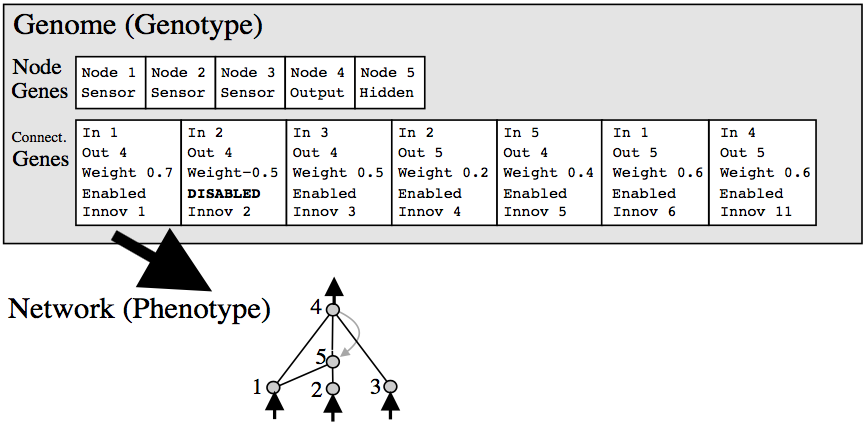
\includegraphics[height=6cm]{slika1}\\
  \caption{Primjer mapiranja genotipa u fenotip \citep{rad2}.}
  \label{slika1}
\end{figure}

\section{Zapis gena}
Postupak genetskog enkodiranja napravljen je tako da se odgovarajući geni lako usklade prilikom križanja jedinki. Genomi su linearna reprezentacija povezanosti unutar mreže (Slika \ref{slika1}). Svaki genom sadrži listu gena veza (eng. \textit{connection genes}), od kojih svaki referencira dva gena čvora (eng. \textit{node gene}) koji su povezani. Geni čvora sadrže listu ulaza, skrivenih čvorova i izlaza koji se mogu spojiti. Svaki gen veze navodi ulazni čvor, izlazni čvor, težinu veze, je li veza uključena i broj inovacije, koji omogućuje lako prepoznavanje odgovarajućih gena.

\begin{figure}[ht]
  \centering
  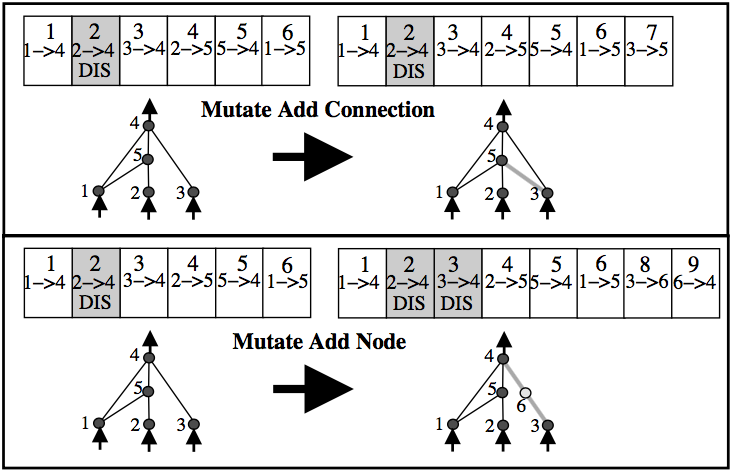
\includegraphics[height=6cm]{slika2}\\
  \caption{Dva tipa strukturalnih mutacija \citep{rad2}.}
  \label{slika2}
\end{figure}

Mutacija u NEAT algoritmu može promijeniti i težinu veza i strukturu mreže. Mutacija težina odvija se kao i kod bilo kojeg neuroevolucijskog sustava, a strukturalna mutacija se odvija na dva načina (Slika \ref{slika2}). Svaka mutacija ekspandira veličinu genoma tako da dodaje gene. U mutaciji dodavanja veze (eng. \textit{add connection mutation}) dodaje se novi gen s nasumično odabranom težinom između dva do tad nepovezana čvora. U mutaciji dodavanja čvora (eng. \textit{add node mutation}) postojeća veza se prepolavlja i postavlja se novi čvor između dva koja su prethodno bila povezana. Stara veza se isključuje i u genom se dodaju dvoje nove veze. Vezi koja ulazi u novonastali čvor postavlja se težina 1, a vezi koja izlazi iz njega dodjeljuje se težina veze koja je isključena prilikom mutacije.

Kroz mutaciju genomi će se postepeno povećavati. To će rezultirati mrežama koje na istim mjestima imaju drugačije veze što može izazvati problem kod križanja. Osim toga, problem nastaje i zbog genoma različite veličine. U nastavku će biti objašnjeno kako NEAT rješava ovaj problem te kako se genomi križaju.

\section{Praćenje gena pomoću povijesnih oznaka}
Sukladno evoluciji sve što sustav treba raditi kako bi znao koji geni su sukladni jest pratiti povijesno ishodište svakog gena. Svaki put kada se pojavi novi gen (kroz strukturnu mutaciju), globalni inovacijski broj (eng. \textit{global innovation number}) se povećava i dodjeljuje tom genu. Samim time, inovacijski broj predstavlja kronologiju svih gena u sustavu.

Mogući problem je da će iste strukturne inovacije dobiti različite inovacijske brojeve u istoj generaciji ako se slučajno dogode više od jednom. Naime, čuvanjem liste inovacija koje su se dogodile u trenutnoj generaciji, moguće je osigurati da se svakoj identičnoj mutaciji dodijeli isti inovacijski broj kada se ista struktura primijeti više od jednom u neovisnim mutacijama unutar generacije.

\begin{figure}[ht]
  \centering
  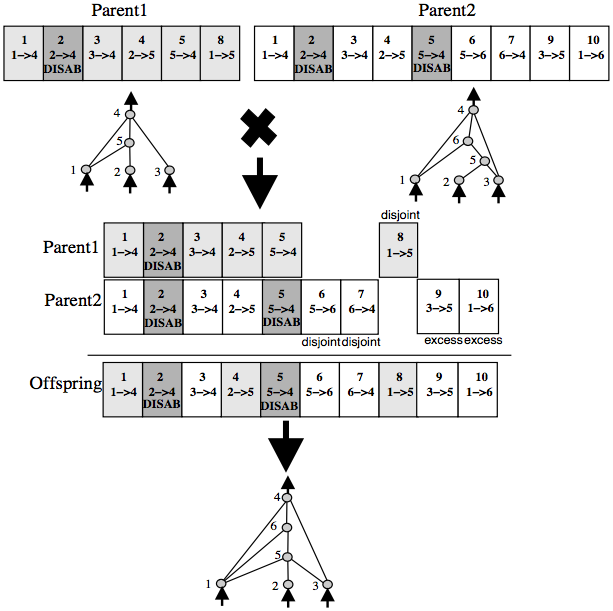
\includegraphics[height=10cm]{slika3}\\
  \caption{Usklađivanje genoma različitih topologija mreža koristeći inovacijske brojeve \citep{rad2}.}
  \label{slika3}
\end{figure}

Sustav sada točno zna koje gene usporediti s kojima (Slika \ref{slika3}). Kod križanja, geni iz oba genoma s istim inovacijskim brojem se usklade. Geni koji se poklapaju (eng. \textit{matching genes}) se nasljeđuju nasumično, dok se geni koji se ne poklapaju u sredini (eng. \textit{disjoint genes}) i geni koji se ne poklapaju na kraju (eng. \textit{excess genes}) nasljeđuju od roditelja s većom dobrotom. Ako im je dobrota ista, također se uzimaju nasumično.

Dodavanjem novih gena u populaciju i križanjem jedinki sustav formira populaciju raznolikih topologija. Naime, populacija sama po sebi ne može održavati topološke inovacije. Zbog toga što se manje strukture optimiziraju brže od velikih i dodavanje čvorova i veza obično inicijalno smanjuje dobrotu mreže, netom izmijenjene strukture imaju male šanse preživjeti više od jedne generacije iako inovacije koje uvode mogu biti presudne za rješavanje zadatka. Rješenje je da se inovacije zaštite tako da se populacije podijeli u vrste, kao što je navedeno u nastavku.

\section{Očuvanje inovacija kroz specijaciju}
Dijeljenjem populacije u vrste gdje su jedinke sa sličnim topologijama daje jedinkama više vremena da optimiziraju strukturu. Na ovaj način čuvaju se inovacije koje bi mogle dugoročno pomoći u dostizanju cilja. Način na koji prepoznajemo slične topologije opet je nešto što treba definirati i tu nam ponovno pomažu povijesne oznake.

Broj neusklađenih gena (eng. \textit{disjoint genes}) i viška gena (eng. \textit{excess genes}) između dvije jedinke je mjera njihove sukladnosti. Što je taj broj veći, dijele manje evolucijske povijesti, znači da su manje kompatibilni. Možemo izračunati kompatibilnu udaljenost (eng. \textit{compatibility distance}) $\delta$ kao funkciju broja viška gena $E$ i neusklađenih gena $D$ te razliku u težinama usklađenih gena $\bar{W}$, uključujući i isključene veze:

\begin{equation}
\delta = \frac{c_1E}{N} + \frac{c_2D}{N} + c_3\cdot\bar{W}
\label{jednakost1}
\end{equation}

Koeficijenti $c_1$, $c_2$ i $c_3$ su parametri kojima definiramo važnost ova tri faktora, a broj $N$ je broj gena u većem genomu i uloga mu je normalizirati izraz.

Jednom kada imamo izračunat $\delta$ određujemo pripadnost vrsti pomoću praga kompatibilnosti (eng. \textit{compatibility threshold}) $\delta_t$. Cijelo vrijeme se održava uređena lista vrsti. Svaka postojeća vrsta predstavljena je nasumičnim genomom unutar vrste iz prethodne generacije. Dani genom \textit{g} u trenutnoj generaciji pozicioniran je u prvu vrstu s kojom je \textit{g} kompatibilan u usporedbi s reprezentativnim genomom te vrste. Na ovaj način vrste se ne preklapaju. Ako \textit{g} nije kompatibilan s nijednom postojećom vrstom, stvara se nova vrsta kojoj se kao reprezentativan uzorak postavlja \textit{g}.

Za reprodukcijski mehanizam koristi se eksplicitno dijeljenje dobrote (eng. \textit{explicit fitness sharing}, Goldberg and Richardson, 1987), gdje organizmi u istoj vrsti moraju dijeliti dobrotu. Tako nijedna vrsta ne može postati prevelika, čak i ako su jedinke dobre. Dakle, teško je da će ijedna vrsta preuzeti cijelu populaciju, što je presudno da bi specijacija funkcionirala. Prilagođena dobrota $f_{i}^{'}$ za organizme $i$ se računa sukladno njihovoj udaljenosti $\delta$ od svakog drugog organizma $i$ u populaciji:

\begin{equation}
f_{i}^{'} = \frac{f_i}{\sum_{j=1}^{n}sh(\delta(i,j))}
\label{jednakost2}
\end{equation}

Funkcija dijeljenja $sh$ je $0$ kada je udaljenost $\delta(i,j)$ veća od praga $\delta_t$, inače je $sh(\delta(i,j))$ postavljena na $1$. Dakle, suma $\sum_{j=1}^{n}sh(\delta(i,j))$ računa broj organizama koji su iste vrste kao i jedinka $i$. Jednom kada se izračuna prilagođena dobrota $f_{i}^{'}$ svih jedinki, uklanjaju se najlošiji organizmi unutar vrsta. Nakon toga, cijela populacija se zamjenjuje potomcima preostalih jedinki u svakoj vrsti.

Razlog iz kojeg se provodi specijacija je da bi se sačuvale topološke inovacije. Zadnja tehnika je da se potraga za rješenjem sustava izvrši što efikasnije. To postižemo minimiziranjem dimenzionalnosti prostora pretrage.

\section{Minimizacija dimenzionalnosti kroz inkrementalni rast iz minimalne strukture}
Idejna preteča NEAT-a, algoritam evolucije topologije i težina umjetne neuronske mreže (eng. \textit{Topology and Weight Evolving Artificial Neural Networks}, \textit{TWEANN}) \citep{rad3}, napunio bi inicijalnu populaciju nasumično generiranim topologijama kako bi potaknuo raznolikost kod završnih rješenja. NEAT traži što manje rješenje i čini pretragu pristranom tako da je inicijalna populacija uniformna, nijedna početna mreža nema skrivenih čvorova. Nova struktura se uvodi postepeno tako što jedinke mutiraju i dobivaju nove čvorove i veze. Novoproširene jedinke preživjet će samo ako imaju dobru dobrotu te zbog toga možemo reći da su sve strukturne promjene u NEAT algoritmu opravdane. Budući da populacija počinje jako mala, dimenzionalnost prostora pretrage je smanjena i NEAT uvijek pretražuje kroz manje dimenzija od ostalih TWEANN algoritama i neuroevolucijskih sustava s fiksnom topologijom. Zbog toga NEAT ima prednost u performansu nad tim algoritmima \citep{rad2}.

\chapter{Neuroevolucija promjenjivih topologija u stvarnom vremenu}
Neuroevolucija promjenjivih topologija u stvarnom vremenu (eng. \textit{Real-time neuroevolution of augmenting topologies}, \textit{rtNEAT}) je metoda bazirana na NEAT algoritmu i predstavljena je u radu Kennetha Stanleya iz 2005. \citep{rad4} gdje se rad algoritam demonstrira u treniranju agenata za igranje igre NERO. Kao većina genetskih algoritama, NEAT je originalno dizajniran da radi \textit{offline}. Jedinke su evaluirane jedna po jedna i tek nakon što se evaluira cijela populacija stvarna se nova populacija koja će formirati sljedeću generaciju. Ključne tri komponente NEAT-a (povijesne oznake, specijacija i minimalne početne strukture) su međuovisne i potrebne su da bi algoritam funkcionirao. U nastavku je objašnjeno kako se ta ideja može nadograditi da bi se izbjegao navedeni problem, tj. da bi algoritam mogao raditi u stvarnom vremenu.

\begin{figure}[ht]
  \centering
  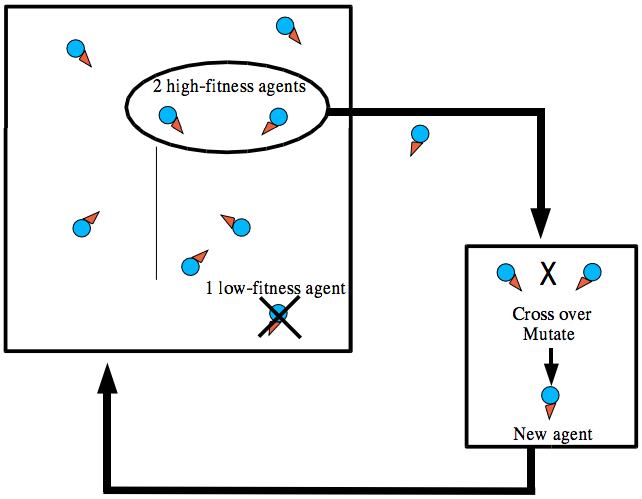
\includegraphics[height=7cm]{slika4}\\
  \caption{Primjer životnog ciklusa \citep{rad4}.}
  \label{slika4}
\end{figure}

\section{Pokretanje NEAT-a u stvarnom vremenu}
U NEAT-u, populacija se zamjenjuje u svakoj generaciji. Zamijeniti cijelu generaciju u stvarnom vremenu bi bilo neprimjereno jer bi se svačije ponašanje promijenilo u istom trenutku. Osim toga, ponašanja bi bila statična tijekom rupa između generacija. Umjesto toga, u rtNEAT-u se organizmi zamjenjuju pojedinačno svakih nekoliko otkucaja (eng. \textit{tick}). Jedna od gorih jedinki se uklanja i zamjenjuje djetetom roditelja koji se biraju među boljim jedinkama. Ovaj ciklus ponavlja se kontinuirano (Slika \ref{slika4}). Pored toga treba sačuvati uobičajeno dinamiku NEAT-a, najviše zaštitu inovacija kroz specijaciju i postepeno nadograđivanje strukture.

Ako je $f_i$ dobrota jedinke $i$, dijeljenje dobrote ga ažurira na $\frac{f_i}{|S|}$, gdje je $|S|$ broj jedinki unutar odgovarajuće vrste. Drugim riječima, dobrota se smanjuje proporcionalno veličini vrste. Ova prilagodba je važna jer se selekcija u rtNEAT-u mora bazirati na prilagođenim dobrotama zato da bi se zadržala ista dinamika kao kod NEAT-a. Dodatno, zato što broj jedinki pridruženih vrsti unutar NEAT-a ovisi o prosječnoj dobroti $\bar{F}$, ovaj broj uvijek mora biti ažuran. Zbog toga, svakih \textit{n} otkucaja sata (igre), rtNEAT izvodi sljedeće operacije:

\begin{enumerate}
  \item Ukloni agenta s najgorom prilagođenom dobrotom (eng. \textit{adjusted fitness}) iz populacije uz pretpostavku da je agent bio živ dovoljno dugo da je ispravno evaluiran.
  \item Ponovno izračunaj $\bar{F}$ za sve vrste.
  \item Izaberi vrstu iz koje će se izabrati roditelji za novog potomka.
  \item Dinamički ažuriraj prag kompatibilnosti $C_t$ i ponovno pridruži agente vrstama.
  \item Uključi novog agenta u populaciju.
\end{enumerate}

Koraci su detaljnije objašnjeni u nastavku.

\subsection{Prvi korak: uklanjanje najgore jedinke}
Cilj ovog koraka je ukloniti loše jedinke, u nadi da će ih zamijeniti nešto bolje. Mreža koja se uklanja se mora pažljivo birati kako bi se očuvala dinamika specijacije. Ako bi uklonili organizam na temelju neprilagođene dobrote, više ne bi mogli zaštititi inovacije, jer bi se nove topologije uklonile čim bi se pojavile. Zbog toga trebamo uklanjati agente s najmanjom prilagođenom dobrotom, zato što prilagođena dobrota u obzir uzima veličinu vrste, tako da se nove male vrste ne maknu čim se pojave.

Važno je ne uklanjati jedinke koje su premlade. U originalnom NEAT-u, dob se ne uzima u obzir budući da se sve mreže evaluiraju približno jednako vremena. U rtNEAT-u to nije tako, jer se novi organizmi konstantno rađaju, što znači da su različiti agenti i različito stari. Bilo bi loše uklanjati jedinke koje su premlade, jer još nisu dovoljno stare da bi mogli točno procijeniti njihovu dobrotu. Zbog toga, algoritam miče samo jedinke koje su žive minimalno \textit{m} jedinica vremena.

\subsection{Drugi korak: Ponovni izračun $\bar{F}$}
Pod pretpostavkom da je bio organizam dovoljno star da ga se ukloni, njegova vrsta sada ima jednog člana manje i zbog toga im se prosječna dobrota (eng. \textit{average fitness}) $\bar{F}$ vjerojatno promijenila. Važno je da $\bar{F}$ bude konstantno ažuran, zato što se $\bar{F}$ koristi za odabir roditeljske vrste u sljedećem koraku. Zbog toga algoritam treba napraviti ponovnu procjenu $\bar{F}$.

\subsection{Treći korak: Odabir roditeljske vrste}
U NEAT-u je broj potomaka $n_k$ dodijeljenih vrsti $k$ jednak $\frac{\bar{F_k}}{\bar{F_tot}}|P|$, gdje je $\bar{F_k}$ prosječna dobrota vrste $k$, $\bar{F_tot}$ suma svih prosječnih dobrota vrsti, a $|P|$ veličina populacije.

Ovaj postupak mora se aproksimirati u rtNEAT-u iako se $n_k$ ne može eksplicitno dodijeliti, budući da se potomci stvaraju jedan po jedan. Pod pretpostavkom da je $n_k$ proporcionalan $\bar{F}$, vrsta koja će biti roditelj se određuje probabilistički:

\begin{equation}
Pr(S_k) = \frac{\bar{F_k}}{\bar{F_tot}}
\label{jednakost3}
\end{equation}

Vjerojatnost odabira vrste da bude roditelj proporcionalna omjeru prosječne dobrote vrste i sumi prosječne dobrote svih vrsti. Tako dugoročno očekujemo da će očekivani broj potomaka svake vrste biti proporcionalan $n_k$, čime zadržavamo dinamiku specijacije originalnog NEAT-a.

\subsection{Četvrti korak: Dinamično mijenjanje praga kompatibilnosti}
U originalnom NEAT-u mreže su dodijeljene vrsti ako su kompatibilne s reprezentativnim pripadnikom vrste. rtNEAT pokušava održati broj vrsta konstantnim tako da prilagođava prag $C_t$, koji određuje je li jedinka kompatibilna s reprezentativnom jedinkom vrste. Kada ima previše vrsta, $C_t$ se povećava tako da vrsti pripadne više jedinki nego što bi inače, a kad ima premalo vrsti, $C_t$ se smanjuje tako da kriteriji za prihvaćanje jedinke u vrstu budu stroži. Prednost ovakvog dinamičnog mijenjanja praga kompatibilnosti (eng. \textit{dynamic compatibility thresholding}) je ta što drži broj vrsti relativno stabilnim.

U rtNEAT-u mijenjanje samo $C_t$ ne može odmah utjecati na broj vrsti, zato što većina populacije jednostavno ostaje gdje je. Samo mijenjanje varijable ne uzrokuje prelazak u drugu vrstu. Zbog toga, nakon što se $C_t$ promijeni cijela populacija se mora ponovno preraspodijeliti u postojeće vrste ovisno o novom $C_t$. Kao i u originalnom NEAT-u, ako mreža ne pripada nijednoj vrsti stvara se nova vrsta kojoj ta mreža postaje reprezentativna jedinka.

\subsection{Peti korak: Zamjena starog agenta s novim}
Budući da se u prvom koraku uklanja jedinka, mora je zamijeniti novi potomak. U trećem koraku odabrana je vrsta iz koje će se birati roditelji potomka.

Ovim korakom završavaju koraci koji su potrebni da bi se NEAT aproksimirao u stvarnom vremenu. U nastavku poglavlja objašnjeno je još kako se definira broj interval izvršavanja petlje, broj otkucaja $n$.

\section{Određivanje broja otkucaja između svake iteracije}
Ako se jedinke zamjenjuju prečesto, ne žive dovoljno duga da se dosegne minimalno vrijeme $m$ potrebno za evaluaciju. S druge strane, ako se agenti zamjenjuju prerijetko, evolucija se previše uspori.

Prikladna frekvencija se može odrediti na konkretan način. Neka je $I$ dio populacije koji je premlad da bio zamijenjen. Kao i prije, $n$ je broj otkucaja između svake iteracije zamjene, $m$ je minimalno vrijeme života i $|P|$ je veličina populacije. Zakon o prihvatljivosti (eng. \textit{law of eligibility}) formuliran je tako da definira koji postotak populacije je premlad jednom kada sustav dosegne konstantno stanje:

\begin{equation}
I = \frac{m}{|P|n}
\label{jednakost4}
\end{equation}

Sukladno prethodnoj jednakosti (\ref{jednakost4}), što su populacija i broj otkucaja veći, manji je postotak premladih jedinki. Tako, rtNEAT može sam odlučiti koliko otkucaja $n$ bi trebalo proći između svake iteracije. Za poželjnu količinu premladih organizama, određenu veličinu populacije i minimalno vrijeme između iteracija imamo:

\begin{equation}
n = \frac{m}{|P|I}
\label{jednakost5}
\end{equation}

Postotak neprihvatljivih jedinki $I$ je hiperparametar algoritma i treba se odabrati tako da odgovara potrebama. Ako je preveliki dio populacije premlad, tj. neprihvatljiv, u svakom trenutku, ne ostavlja se dovoljno veliki izbor kod odabira jedinki za križanje. Jednakost \ref{jednakost5} omogućuje dobivanje točnog broja otkucaja $n$ kako bi se održao željeni postotak prihvatljivosti.

Izvodeći dane operacije svakih $n$ otkucaja, odabirom dobrih jedinki za uklanjanje i mijenjanjem istih potomkom pažljivo odabranom vrstom, rtNEAT replicira NEAT u stvarnom vremenu. Zbog toga je NEAT sada moguće ubaciti u računalnu igru i dobiti agente koji će kroz trajanje igre postajati sve kompleksniji \citep{rad4}.

\chapter{Primjena neuroevolucijskih algoritama u igri \textit{StarCraft: Brood War}}
Element igre u kojem će se razmatrati korištenje ovih algoritama je mikromenadžment (eng. \textit{micromanagement}), presudna komponenta \textit{RTS} igara koja predstavlja upravljanje borbom unutar igre. Mikromenadžment uključuje donošenje odluka kao što su: hoće li određena jedinka započeti borbu sa suparničkim jedinkama, hoće li je nastaviti ili će pobjeći te kako će se gibati i koje će protivnike fokusirati prilikom zadavanja udaraca.

\citep{rad1} koristi rtNEAT mrežu za mikromenadžment i unutar 300 generacija ostvaruje veliku stopu pobjeda. Rad navodi da algoritam dopušta brzu adaptaciju i razvoj strategije u stvarnom vremenu. Ograničenje je što se za evaluaciju koristila prilagođena mapa koja je uvela nerealan uvjet koji momentalno nadoknađuje izgubljene jedinke što se inače ne događa u pravim partijama. U danom primjeru svejedno se vidi potencijal korištenja neuroevolucijskih algoritama u \textit{SC:BW}. \citep{rad5} idejno nastavlja prethodni rad i koristeći slične postavke testira učinkovitost NEAT i rtNEAT algoritama u dva eksperimenta. U nastavku je opisano programsko ostvarenje \citep{rad5} te su navedeni njihovi rezultati.

\begin{figure}[ht]
  \centering
  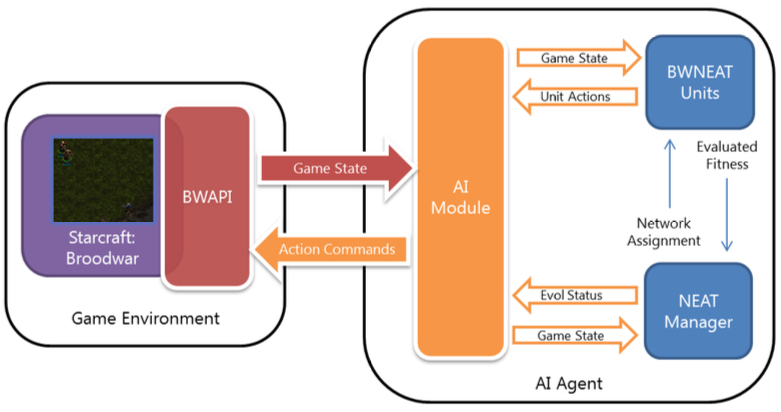
\includegraphics[height=6cm]{slika5}\\
  \caption{Pregled arhitekture \citep{rad5}.}
  \label{slika5}
\end{figure}

\section{Programsko ostvarenje}
Arhitektura je prikazana na slici \ref{slika5}. Brood War API (BWAPI) je programski okvir otvorenog koda (eng. \textit{open source framework}) za izvedbu i pokretane AI modula unutar StarCraft igre. On ima funkcionalnost da dobiva informacije o stanju igre i da zadaje naredbe jedinicama u igri. Te jedinice su enkapsulirane kao BWNEAT jedinice (eng. \textit{BWNEAT Units}), s pratećom neuronskom mrežom za donošenje odluka. NEAT menadžer (eng. \textit{NEAT manager}) je odgovoran za instanciranje BWNEAT jedinica i sučelje je za NEAT i rtNEAT algoritme. Za rtNEAT broj otkucaja $n$ između svake je 50.

\begin{figure}[ht]
  \centering
  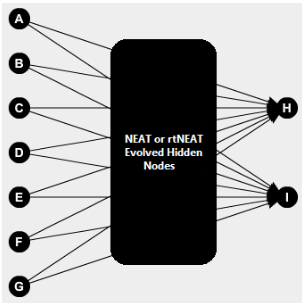
\includegraphics[height=7cm]{slika6}\\
  \caption{Inicijalna struktura umjetne neuronske mreže \citep{rad5}.}
  \label{slika6}
\end{figure}

\subsection{Arhitektura neuronske mreže}
Inicijalna arhitektura mreže prikazana je na slici \ref{slika6}. U ovom primjeru odluke koje se donose su jako jednostavne, mreža ne temelju dobivenih informacija, koje se smatraju relevantnima za donošenje odluke, odlučuje hoće li se boriti \textit{H} ili će pobjeći \textit{I}. Informacije koje mreža dobiva su, redom od \textit{A} do \textit{G}: pristranost (eng. \textit{bias}), vrijeme kad će se ponovno moći koristiti oružje (eng. \textit{weapon cooldown}), preostala količina života (eng. \textit{remaining health}), doseg oružja (eng. \textit{weapon range}), doseg oružja neprijateljske jedinice (eng. \textit{enemy weapon range}), broj prijateljskih jedinica u dosegu (eng. \textit{num allies in range}), broj neprijateljskih jedinica u dosegu (eng. \textit{num enemies in range}). Ako se jedinica odluči boriti, jedinica napadne neprijateljsku s najmanje preostalog života unutar dosega svog oružja, a ako se odluči povući, jedinica će se pomoću težinskog vektora pomaknuti za malu udaljenost dalje od neprijatelja i prepreka.

\subsection{Funkcija dobrote}
Budući da funkcija dobrote treba reflektirati performans jedinice, definiramo ga kao:

\begin{equation}
F_i = \frac{TDD_i - HPL_i}{IHP_i} + 1
\label{jednakost6}
\end{equation}

Funkcija uzima u obzir totalnu štetu koju je jedinica nanijela (eng. \textit{total damage dealt}) $TDD$, gubitak jedinica života tokom partije (eng. \textit{hit point loss}) $HPL$ i početnu količinu jedinica života (eng. \textit{initial hit point}) $IHP$.

\section{Eksperimenti}
U primjeru danom u radu \citep{rad4} uspoređuju se četiri varijacije jedinica. Dvije vrste jedinica u \textit{SC:BW} su \textit{melee} (jedinice koje se bore iz blizine) i \textit{ranged} (jedinice koje se bore na daljinu). Dakle, četiri varijacije u kojima se isprobavao performans algoritama su: \textit{melee} protiv \textit{melee}, \textit{melee} protiv \textit{ranged}, \textit{ranged} protiv \textit{melee} i \textit{ranged} protiv \textit{ranged}. Razlog zašto se koriste ovakve varijacije je kako bi se simulirali različiti scenariji mikromenadžmenta. Broj jedinica je fiksnih 12 protiv 12 jedinica koje upravlja računalo te se koristi prilagođena plosnata mapa.

\subsection{Eksperiment evolucijskog procesa}
U prvom eksperimentu oba algoritma su se testirala u 300 generacija za sve četiri varijacije. Svaka partija ponovljena je 25 puta kako bi se smanjio utjecaj nasumičnosti. Na kraju se gleda tko je pobijedio, algoritam ili računalo. Po rezultatima se ne može reći da je ijedan algoritam kategorički bolji. Postotak pobjede je veći za NEAT u varijacijama s različitim tipovima jedinica (\textit{melee} protiv \textit{ranged} i \textit{ranged} protiv \textit{melee}), a za rtNEAT u preostale dvije varijacije (\textit{melee} protiv \textit{melee} i \textit{ranged} protiv \textit{ranged}). Rezultati su prikazani na slici \ref{slika7}.

Razlog zašto su algoritmi toliko bolji u varijacijama gdje igraju s \textit{ranged} jedinicama je taj što mreže nauče neke sofisticirane tehnike kao što su \textit{hit-and-run}, gdje jedinica udari neprijateljsku jedinicu i miče se od nje dok ne može ponovno koristiti oružje, time izlazi iz dosega neprijateljskoj jedinici i smanjuje vjerojatnost da će ona uspješno uzvratiti udarac. Ova tehnika nije tako efikasna kod \textit{melee} jedinica zato što je njihov mali u odnosu na \textit{ranged} jedinice i zbog toga, ako se \textit{melee} jedinica počne odmicati, više ne može udariti neprijateljsku jedinicu jer je i mali korak stavlja predaleko za uspješan udarac.

\begin{figure}[ht]
  \centering
  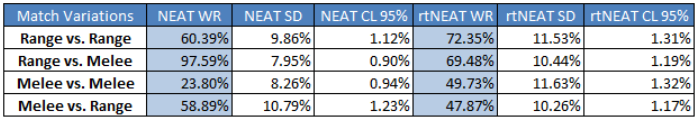
\includegraphics[height=2cm]{slika7}\\
  \caption{Rezultati prvog eksperimenta \citep{rad5}. Postotak pobjede (eng. \textit{win rate}) WR i standardno odstupanje (eng. \textit{standard deviation}) SD i interval pouzdanosti (eng. \textit{confidence level}) CL.}
  \label{slika7}
\end{figure}

\subsection{Eksperiment generacijske konvergencije}
U ovom eksperimentu algoritmi su postavljeni da se zaustave nakon 1000 generacija ili kada nađu rješenje koje pobjedi 10 puta zaredom, sve ostale postavke iste su kao i u prethodnom eksperimentu. Kada kandidat pobijedi prvi put zaustavlja se evolucija i igraju se partije dok ne pobijedi 10 puta zaredom ili jednom ne izgubi, kada se evolucija nastavlja. Kao rezultat se gleda prosječan broj generacija koji je bio potreban da bi se razvilo zadovoljavajuće rješenje. Ni za jednu varijaciju nije bilo potrebno više od oko 100 generacija da dosegne zadovoljavajuće rješenje. Rezultati su prikazani na slici \ref{slika8}. NEAT konvergira brže za varijacije s različitim tipovima jedinica, dok rtNEAT konvergira brže u preostale dvije varijacije. NEAT ima puno veće oscilacije u prosječnom broju generacija za različite varijacije od rtNEAT-a, što bi moglo sugerirati da je rtNEAT stabilniji \citep{rad5}.

\begin{figure}[ht]
  \centering
  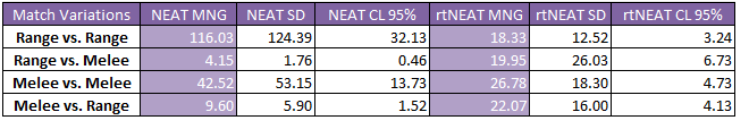
\includegraphics[height=2cm]{slika8}\\
  \caption{Rezultati drugog eksperimenta \citep{rad5}. Srednji broj generacija (eng. \textit{mean number of generations}) MNG, standardno odstupanje (eng. \textit{standard deviation}) i interval pouzdanosti (eng. \textit{confidence level}) CL.}
  \label{slika8}
\end{figure}

\chapter{Zaključak}
Sveukupno, eksperimenti su pokazali da su oba algoritma sposobna generirati rješenja efikasna u mikromenadžmentu protiv uobičajene \textit{SC:BW} umjetne inteligencije \citep{rad5}. Ono što se može primijetiti u ovom eksperimentu je da su jedinice, koje su se naučile bježati od borbe dok ne uoče prijateljske jedinice kako se bore i odluče pomoći, imale veću dobrotu od onih koje su bezuvjetno ulazile u borbu. To se događalo zbog toga što su jedinice, koje su u početku bježale, na kraju imale manji gubitak životnih bodova, što ih je činilo povoljnijim rješenjem. Problem je što je to na kraju dovelo do toga da su nakon niza generacija ostale samo jedinice koje bi konstantno samo bježale i zbog toga izgubile partiju.

Evolucija u stvarnom vremenu je brža u uvođenju promjena koje inicijalno smanjuju dobrotu, ali time dobiva robusniju konvergenciju prema rješenju neovisno o tipovima jedinica o kojima se radi. To je zbog toga što, zbog komponente stvarnog vremena, može puno brže odgovarati na podražaje koje dobije i promjene koje osjeti. Algoritam bi se mogao nadograditi tako da se poveća broj parametara koji se uvode u mrežu ili poveća broj odluka koje jedinica može donijeti. Na primjer, jedinica bi mogla primati preciznije podatke ne samo o poziciji nego i o orijentaciji, a izlaz bi moglo biti i pomicanje u nekom određenom smjeru, što bi jedinicu moglo postaviti u bolju poziciju za sljedeći napad. Odabir mete je kompleksan zadatak sam za sebe i mogao bi se učiti odvojenom mrežom, zato što jedinice različitih tipova imaju prednost nad određenim jedinicama, što bi na kraju krajeva ovime mogli i naučiti.

Rezultati \citep{rad5} su pokazali obećavajuću učinkovitost umjetne inteligencije koja uči nad onom koja je skriptirana.

\bibliography{literatura}
\bibliographystyle{fer}

\chapter{Sažetak}
Kratak pregled NEAT (eng. neuroevolution of augmenting topologies) i rtNEAT (eng. real-time neuroevolution of augmenting topologies) algoritama te koje su novitete uveli. Diskusija kako se ti algoritmi mogu koristiti u treniranju umjetne inteligencije za igranje RTS igara. Konkretno prikazano na primjeru igre \textit{StarCraft: Brood War}.

\end{document}